\documentclass{hw}
\usepackage{xcolor}
\usepackage{enumitem}
\usepackage{graphicx}
\usepackage{caption}
\usepackage{subcaption}

\usepackage{listings}
% STUDENTS: Please fill these out with your information
\newcommand{\name}{Fill Here}
\newcommand{\netid}{Fill Here}
\newcommand{\collaborators}{Fill Here}
% / STUDENT

\newcommand{\hwnum}{3}
\newcommand{\duedate}{November 7, 11:59pm ET}
\renewcommand{\title}{Dynamic programming and randomized algorithms}
\newcommand{\io}{\textbf{Code input and output format.} }

\newcommand{\submission}{\textbf{Submission.}}

\lstset{
  basicstyle=\ttfamily\scriptsize,    % Use a scriptsize typewriter font
  breaklines=true,               % Break long lines
  frame=single,                  % Frame the code block
  numbers=left,                  % Add line numbers on the left
  numberstyle=\tiny\color{gray}, % Make line numbers small and gray
  keywordstyle=\color{blue},     % Color keywords blue
  commentstyle=\color{green},    % Color comments green
  stringstyle=\color{red},       % Color strings red
}
\newtheorem{claim}{Claim}

\begin{document}

%%%%%%%%%%%%%%%%%%%%%%%%%%%%%%%%%%%%%%%%%%%%%%%%%%%%%%%%%%%%%%%%%%%%%%%%%%%%%%%%
% Problem 1: Bipartite Graphs


\begin{problem}
This problem involves working with graphs, specifically focusing on bipartite properties and matching. 

\begin{subproblem}
Test if a given graph is bipartite using the Breadth First Search (BFS) approach.

Given the function \texttt{is\_bipartite(g\_l) -> bool}, the purpose is to determine if the graph represented by the adjacency dictionary \texttt{g\_l} is bipartite or not. A simple BFS algorithm can be employed where nodes are colored in a way that no two adjacent nodes share the same color. If it's possible to color the graph using two colors in this way, the graph is bipartite.

(\textit{10 points}) Implement the \texttt{is\_bipartite} function in \texttt{problem\_1/p1\_a.py}.
\end{subproblem}

\io The input for \textbf{Problem 1 (a)} is a graph represented as an \textbf{adjacency dictionary} (see Listing \ref{lst1a:codeblock}), and the output should be a Boolean (True if the graph is bipartite, False otherwise).

\begin{lstlisting}[language=Python,caption={The adjacency dictionary representation, where the keys represent a node, and the value list represents the nodes the `key' node is connected to.},label={lst1a:codeblock},captionpos=b]
{0:[1,3], 1:[0,2], 2:[1,3], 3:[0,2]}. 
\end{lstlisting}

\begin{subproblem}
Determine the maximal bipartite match of a given bipartite graph.

For the function \texttt{maximal\_bipartite\_match(g) -> int}, the objective is to find the maximum number of matches that can be achieved in the bipartite graph represented by the adjacency matrix \texttt{g}.

(\textit{10 points}) Implement the \texttt{maximal\_bipartite\_match} function in \texttt{problem\_1/p1\_b.py}.
\end{subproblem}

\io The input for \textbf{Problem 1 (b)} is a bipartite graph represented as an \textbf{adjacency matrix} (see Listing \ref{lst1b:codeblock}). The output should be an integer representing the number of maximal matches.
\begin{lstlisting}[language=Python,caption={The adjacency matrix representation, where an entry $i,j$ is 1 if there is an edge between nodes $i$ and $j$, 0 otherwise.},label={lst1b:codeblock},captionpos=b]
[[0, 1, 0, 1], [1, 0, 1, 0], [0, 1, 0, 1], [1, 0, 1, 0]]. 
\end{lstlisting}

\end{problem}

\begin{solution}
Please submit functional code. No written component for this problem :)
\end{solution}

\newpage

%%%%%%%%%%%%%%%%%%%%%%%%%%%%%%%%%%%%%%%%%%%%%%%%%%%%%%%%%%%%%%%%%%%%%%%%%%%%%%%%
% Problem 2

\begin{problem}
In a futuristic digital city, there are $n$ data hubs and $k$ service providers that need to be interconnected. As an input, you are given the number of data hubs and service providers and a dictionary \texttt{connections} showing which data hubs \textit{can be connected} to which service providers. You are also given \texttt{provider$\_$capacity} showing \textit{how many connections} each service provider can handle, and \texttt{preliminary\_assignment} which has the assignment for all the other hubs except the last one. These variables are shown in the example code snipped in Listing~\ref{lst2:codeblock_l}. In this problem, data hubs are labelled $0, 1,..., n-1$ and service providers are labelled $n, n+1,..., n+k-1$.
\\
\begin{lstlisting}[language=Python,caption={The python function call to be made to generate the graphs for Problems 2.a,b,c.},label={lst2:codeblock_l},captionpos=b]
plan_city_a(num_data_hubs = 5,
            num_service_providers = 5,
            connections = {0: [5,7,8], 1: [5, 8], 2: [7,8,9], 3: [5, 6, 8, 9], 4: [5,6,7,8]},
            provider_capacities = [0]*5 + [0,1,0,2,2],
            preliminary_assignment = {0: 8, 1: 8, 2: 9, 3: 9})
\end{lstlisting}

Your task is to ensure each data hub is connected to a service provider while considering capacity constraints. If the last hub ($n-1$) can't be connected, find out which service provider's capacities need to be increased by one for a feasible solution.

To solve this, you will make use of a graph-based approach and the Ford-Fulkerson algorithm. In this graph, the source is a vertex from which flow starts, and the sink is the one where flow ends. The source will be connected to each data hub and each service provider to the sink. If a data hub can be connected to a service provider, there will be a directed edge between them in the graph. The capacity of the edges from the source to each data hub, as well as the capacity of each edge from a data hub to its possible service providers, is 1. The capacity from service providers to the sink is based on \texttt{provider$\_$capacity}. In this problem, constructing the residual graph correctly is extremely important. Therefore, part (a), (b) and (c) will focus on an incremental approach to building the correct graph. \textbf{Part (a), (b) and (c) are to be implemented in the function \texttt{plan\_city\_a} in \texttt{problem$\_$2/p2$\_$a.py}}. 

Note that in the example shown in Listing~\ref{lst2:codeblock_l}, since there are only 5 service providers, we assign a capacity of `0' to the 5 data hubs for convenience in implementation. Thus \texttt{provider\_capacities} is to be described as [0]*\texttt{num\_data\_hubs} (5 in this example) + list(\texttt{service\_provider\_capacity}).

\begin{subproblem}
(\textit{5 points}) Generate the first part of the visualization graph showing connectivity from the source to data hubs to the service providers, based on the given connections dictionary. Implement this in \texttt{problem$\_$2/p2$\_$a.py}. Generate the graph using the input shown in Listing~\ref{lst2:codeblock_l} and provide the visualization with the caption (Problem 2.a.) in the write-up.
\end{subproblem}

\begin{subproblem}
(\textit{5 points}) Extend the graph by connecting the service providers to the sink using the given provider$\_$capacity. Implement this in \texttt{problem$\_$2/p2$\_$a.py}. Generate the graph using the input shown in Listing~\ref{lst2:codeblock_l} and provide the visualization with the figure caption (Problem 2.b.) in the write-up.
\end{subproblem}

\begin{subproblem}
(\textit{10 points}) Using the graphs from the previous parts, create the residual graph. This graph will help in determining the feasible flow of connections. Implement this in \linebreak \texttt{problem$\_$2/p2$\_$a.py}. Generate the graph using the input displayed in Listing~\ref{lst2:codeblock_l} and provide the visualization with the figure caption (Problem 2.c.) in the write-up.
\end{subproblem}

\begin{subproblem}
(\textit{10 points})
Implement the algorithm to determine if each data hub can be connected to a service provider. Return \texttt{`True'} if each data-hub can be connected to a service provider, otherwise return \texttt{`False'}. Implement this in \texttt{problem$\_$2/p2$\_$d.py}. Note that you can simply copy paste the code for the residual graph generation from \texttt{problem$\_$2/p2$\_$a.py} and focus on the rest of the algorithmic implementation.
\end{subproblem}

\begin{subproblem}
(\textit{20 points})
Extend the implementation to now provide the final connectivity map if it is feasible. If it is not feasible, the output should be a list of zeros for each data hub, followed by a list of $0$s and $1$s indicating which service providers capacities should be increased by one for a feasible solution. Implement this in \texttt{problem$\_$2/p2$\_$e.py}. Note that you can simply copy paste the code from \texttt{problem$\_$2/p2$\_$d.py} and focus on the rest of the algorithmic implementation.
\end{subproblem}


\end{problem}
\begin{solution}
Please attach figures in Figure \ref{fig:three_images}

\begin{figure}[h!]
    \centering
    
    \begin{subfigure}{.32\textwidth}
        \centering
                \fbox{\parbox[b][4cm][c]{0.95\linewidth}{\centering P2.a Graph}} % Placeholder box with 'text'

        \caption{Problem 2.a.}
    \end{subfigure}%
    \hfill
    \begin{subfigure}{.32\textwidth}
        \centering
                \fbox{\parbox[b][4cm][c]{0.95\linewidth}{\centering P2.b Graph}} % Placeholder box with 'text'

        \caption{Problem 2.b.}
    \end{subfigure}%
    \hfill
    \begin{subfigure}{.32\textwidth}
        \centering
                \fbox{\parbox[b][4cm][c]{0.95\linewidth}{\centering P2.c Graph}} % Placeholder box with 'text'

        \caption{Problem 2.c.}
    \end{subfigure}
    
    \caption{The generated graphs for the problems 2.a, 2.b and 2.c.}
    \label{fig:three_images}
\end{figure}
\end{solution}
\newpage

%%%%%%%%%%%%%%%%%%%%%%%%%%%%%%%%%%%%%%%%%%%%%%%%%%%%%%%%%%%%%%%%%%%%%%%%%%%%%%%%
% Problem 3


\begin{problem}
Dr. Heinz Doofenshmirtz has just discovered a secret product studio idea in the Bloomberg Masters Studio and is making his way to the Tata Innovation Center to present it. Perry the Platypus from a rival start-up aims to intercept Dr. Heinz Doofenshmirtz by blocking the paths to the Tata Innovation Center. Determine the fewest number of paths that Perry the Platypus should block so that there's no path between Masters Studio and Tata.
\begin{figure}
    \centering
    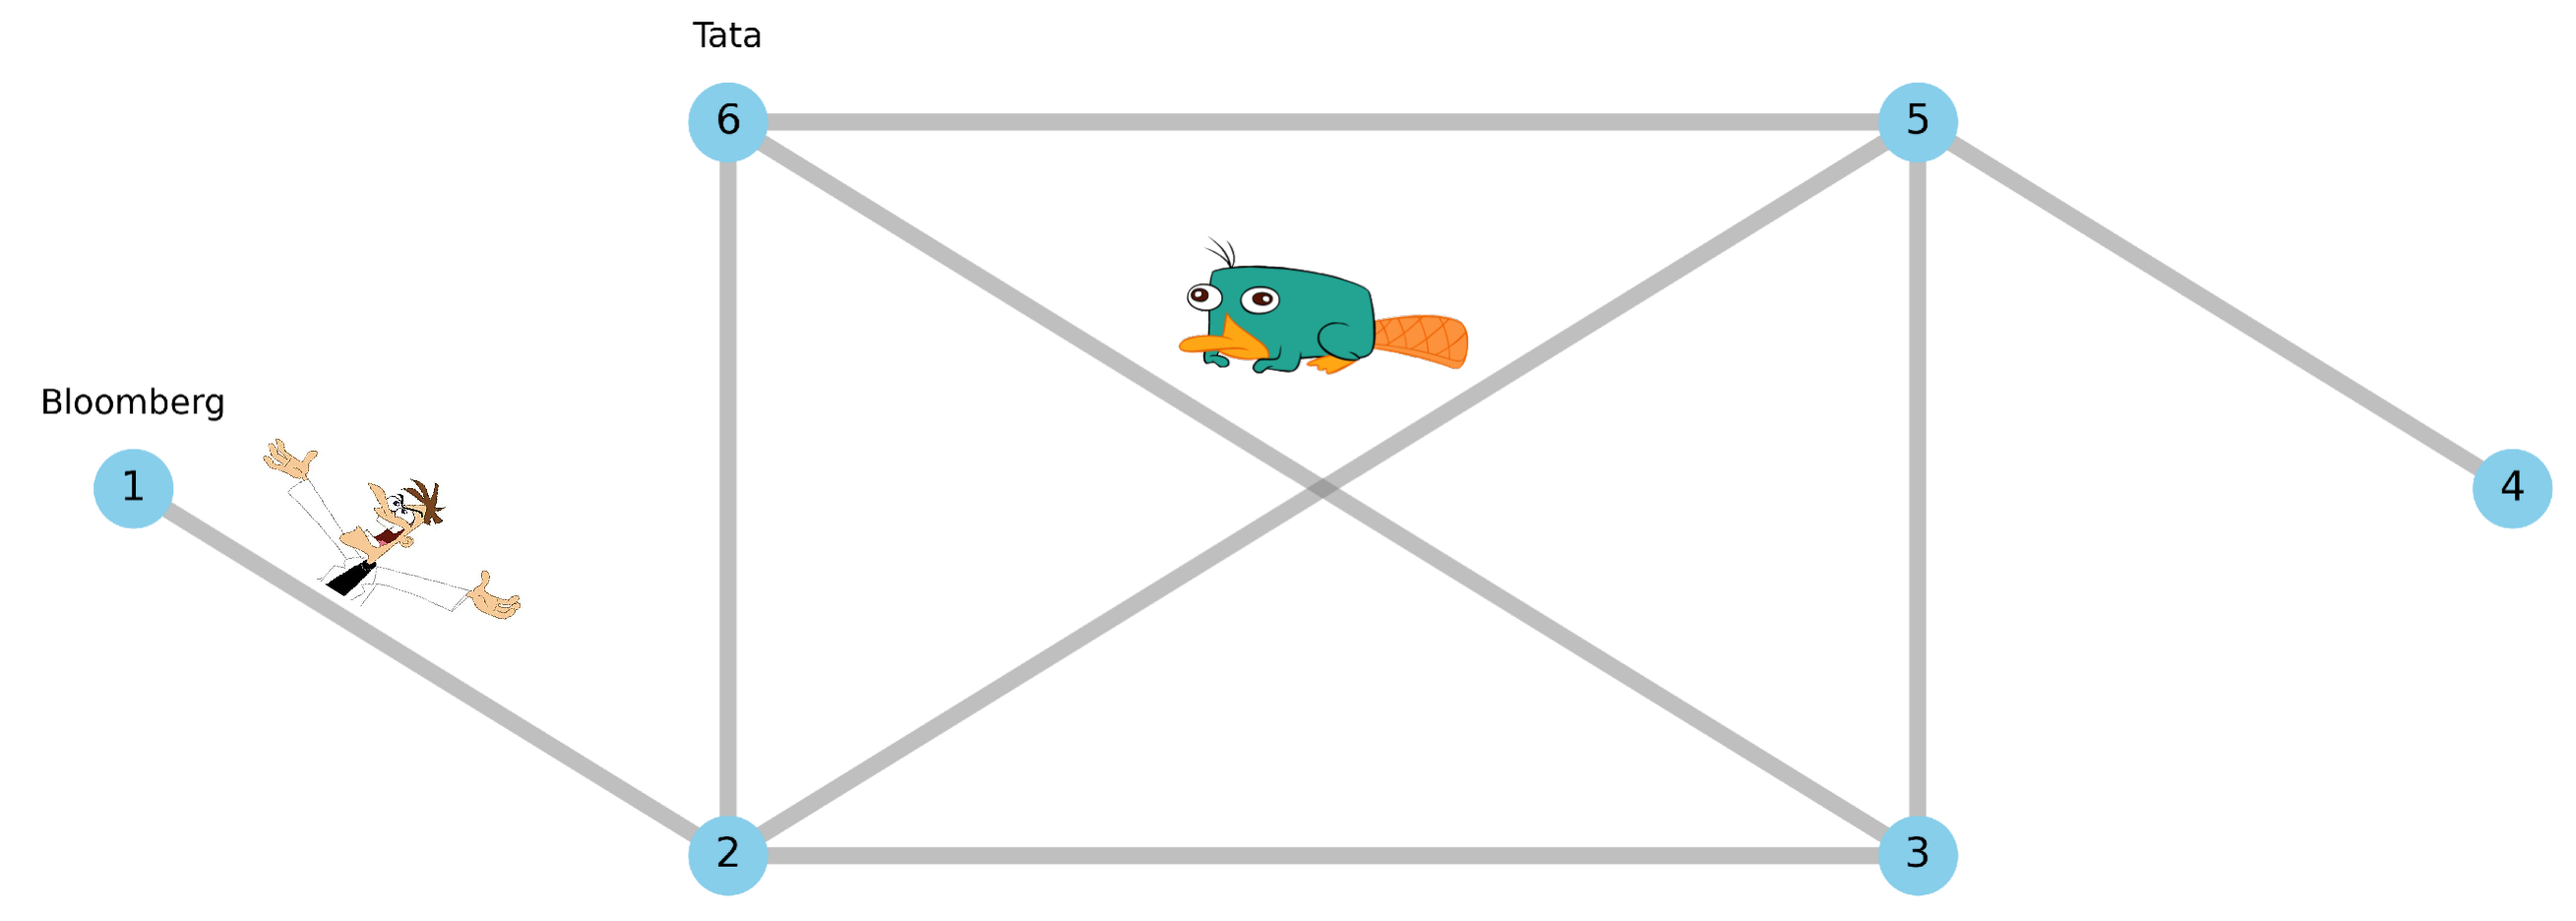
\includegraphics[width=\columnwidth]{figures/edited.png}
    % \caption{Caption}
    \label{fig:enter-label}
\end{figure}
\begin{subproblem}
(\textit{30 points})
    Compute the minimal number of paths to be blocked by Perry the Platypus. 
\end{subproblem}

% \begin{subproblem}
% (\textit{20 points})
%     Return a list of \textit{r} items, where each item indicates which passages need to be blocked. 
% \end{subproblem}

\io You are to design a function called \texttt{find\_paths} with the following inputs:
\begin{itemize}
    \item $n$, which correspond to the total number of junctions. The junctions are numbered from 1 to $n$, Dr. Heinz Doofenshmirtz is at the masters studio, which is at junction 1. Tata Innovation Center is at junction $n$. 
    \item paths: A list of tuples, where each tuple contains two integers---$x$ and $y$---indicating a passage between junctions $x$ and $y$. All paths are accessible in both directions, and there is at most one passage between two junctions.
\end{itemize}

\textbf{Examples:}
\begin{itemize}
\item For $n$ = 5, paths = [(1,2), (3,4), (1,5), (2,5)], the paths (1,2) and (1,5) or (2,5) and (1,5) need to be blocked off to ensure product studio failure. The output should be 2.
\item For $n$ = 12, paths = [(1,4), (1,8), (1,9), (8, 9), (9, 12), (8, 11), (8, 12), (3,4), (3, 12), (1,5), (2,5)], three paths, such as (1, 4), (1, 8), (1, 9), need to be blocked off to ensure product studio failure. The output should be 3.
\end{itemize}
\end{problem}

\begin{solution}
Please submit functional code. No written component for this problem :)
\end{solution}

\newpage

\begin{challenge}
You and your \(n\) friends have a collection of cards from the hit card game One! Each card has a numeric value, ranging from 1 to \(m\), and each card belongs to one of \(k\) colors, which we represent as numbers between 1 and \(k\) for convenience. So a card is a tuple \((x, c)\) where \(x \in \{1, \dots , m\}\) is its numeric value, and \(c \in \{1, \dots , k\}\) is its color.

We can represent a regular 52-card deck by taking \(m = 13\) and \(k = 4\), with Ace representing the numeric value 1, Jack being 11, Queen being 12, and King being 13, and clubs being suit 1, diamonds being 2, hearts being 3 and spades being 4.

To keep track of the number of cards you have over multiple decks, you and your friends decide to make stacks out of the cards. The stacks have to meet the following constraints:
\begin{itemize}
    \item Every stack has to start with the lowest card (value 1) and end with the highest (value \(m\)).
    \item Within each stack, each card \((x, c)\) can be followed by card \((x', c')\) in the following cases:
    \begin{itemize}
        \item if the next card is of the same color and the next higher value (that is, \(c' = c\) and \(x' = x + 1\)),
        \item if the next card is of any different color and the same value (that is, \(c'\) can be anything, and \(x' = x\)).
    \end{itemize}
\end{itemize}

Each of you will get some cards (not necessarily the same number of cards each). You are seated around a table and you label the people clockwise from \(i = 1\) to \(n\). Turns are done in the following way:
\begin{itemize}
    \item Any person can start the next stack, by putting one or more cards (according to the rules described above).
    \item Once the stack has been started by person \(i\), you take turns in increasing circular order placing cards on the stack following the rules described above (so the next person to place a card will be \((i + 1) \mod n\)).
    \item You and your friends continue taking turns this way until the stack is complete.
    \item Each person can play multiple cards, but at least one card must be played each turn.
\end{itemize}

Naturally, each card can only be part of one stack.

\io You are to design a function called cards\_game with the following inputs:
\begin{itemize}
    \item m, n and k correspond to the range of the cards numeric value (1,..., m), the number of friends (n) and the number of colors (k).
    \item counts is a dictionary where for each 'friend' as the dictionary key, we have a tuple (a, b) indicating the cards numeric value and color respectively.
\end{itemize}

\textbf{Example:}

Let \(m = 3\), \(k = 2\) and \(n = 3\), and suppose you and your friends have the following cards:

Person 1: \((1,2)\), \((3,2)\)

Person 2: \((1,1)\), \((2,1)\), \((2,2)\)

Person 3: \((2,2)\), \((3,2)\)

Thus, the function call would be: 

\begin{lstlisting}[language=Python,caption={The python function call to be made to generate the graphs for Problems 2.a,b,c.},captionpos=b]
cards_game(m=3, k=2, n=3, counts = {1: [(1,2),(3,2)], 2: [(1,1), (2,1), (2,2)], 3: [(2,2), (3,2)]})
\end{lstlisting}

Then we can make two stacks:
\begin{itemize}
    \item Person 1 places \((1,2)\); person 2 places \((2,2)\); person 3 places \((3,2)\)
    \item Person 2 places \((1,1)\), \((2,1)\); person 3 places \((2,2)\); person 1 places \((3,2)\).
\end{itemize}

For the following input:

Person 1: \((1,2)\), \((2,2)\), \((2,2)\), \((3,2)\)

Person 2: \((1,1)\), \((2,1)\)

Person 3: \((3,2)\)


The function call would be: 

\begin{lstlisting}[language=Python,caption={The python function call to be made to generate the graphs for Problems 2.a,b,c.},captionpos=b]
cards_game(m=3, k=2, n=3, counts = {
                    1: [(1,2), (2,2), (2,2), (3,2)],
                    2: [(1,1), (2,1)],
                    3: [(3,2)]})
\end{lstlisting}

Only one stack is possible.

Given the cards held by you and each of your friends (where not all possible cards are necessarily present, and there may also be duplicates), implement a polynomial-time algorithm to find out the maximum number of stacks you can create from your cards. Implement it in  \texttt{challenge$\_$1/cards$\_$a.py}.

\textbf{A little help to get you started:}
\begin{itemize}
    \item Our current topic is network flows, so think about whether you can reduce the stated problem to the maximum flow problem.
    \item Setting up good notation to express what you want to achieve is a good first step to help you think about this! Because of the rules of the game, it seems sensible to represent a card as \((i, x, c)\) where \(i\) is the person holding the card, \(x\) is the card’s value, and \(c\) is the card’s suit. What can you say about a card \((i', x', c')\) if it is possible to place it on top of \((i, x, c)\)?
\end{itemize}
\end{challenge}

\begin{solution}

Please submit functional code. No written component for this problem :)
\end{solution}


\end{document}
